\chapter{Introduction}\label{chap:introduction}

\section{Motivation}
Instance detection is a fundamental challenge in computer vision with critical applications in fields ranging from autonomous driving to medical imaging. Recent advancements have seen a shift from traditional Convolutional Neural Networks (CNNs) to the transformative capabilities of Transformers, as demonstrated by Dosovitskiy et al. (2020) with their Vision Transformer (ViT)~\cite{dosovitskiy2020image}. Subsequently, the concept of utilizing deep ViT features as dense visual descriptors was introduced by Amir et al. (2021)~\cite{amir2021deep}, highlighting the strong semantic information these descriptors provide about instances within an image. This shift highlights a growing interest in leveraging deep, self-supervised features for dense visual representation.

In this context, the current state-of-the-art method for unsupervised instance segmentation, CutLER~\cite{wang2023cut}, utilizes DINO features~\cite{caron2021emerging} to identify instances within images. Despite its advancements, CutLER faces challenges such as grouping of nearby instances and complex background patterns. Addressing these issues not only aims to improve the practical performance of unsupervised methods but also contributes to understanding the efficacy of self-supervised features and the role of inductive biases in computer vision. These methods are crucial not only for their direct applications but also as pre-training techniques for downstream tasks, enhancing models trained with limited labeled data.

This thesis seeks to investigate and overcome these limitations by analyzing the CutLER baseline and proposing possible enhancements to unsupervised object detection and segmentation. By improving these methods, we aim to advance the state of unsupervised learning, providing deeper insights into feature representations and their impact on vision tasks.

%\input{Images/main/mask_cut_cutler_comparison}
\begin{figure*}
	\centering
	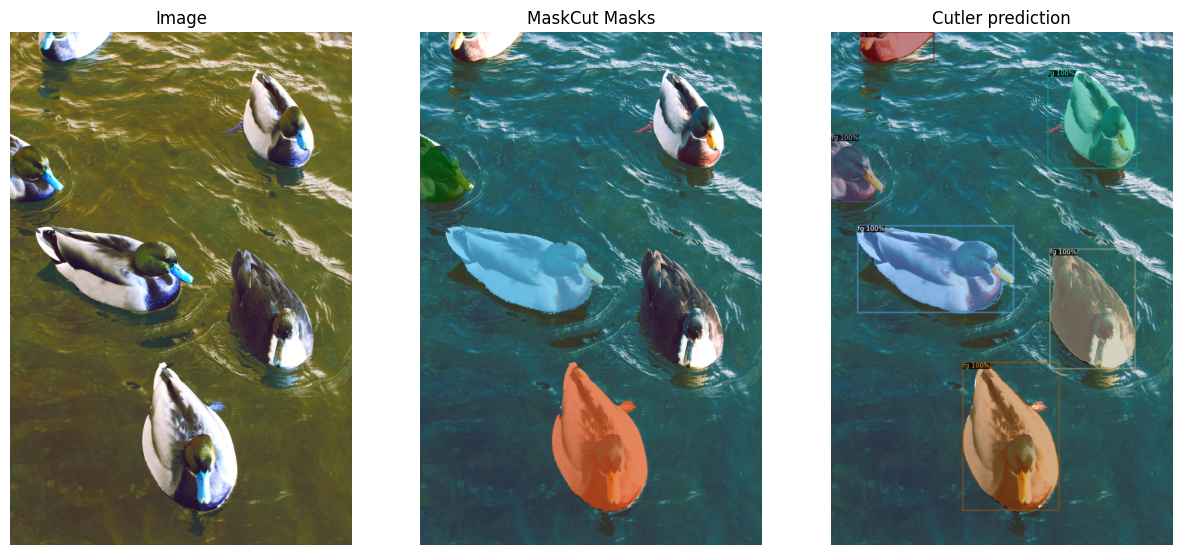
\includegraphics[width=1\textwidth]{Images/main/intro_cutler_pic.png}
	\caption[\textbf{Comparison of MaskCut and CutLER outputs}]{\textbf{Maskcut and CutLER outputs}. Figure illustrates the outputs of CutLER and MaskCut with N=3(Number of masks generated).}
	\label{fig:mask_cut_cutler_comparison}
\end{figure*}

\section{Overview of CutLER}
In the field of unsupervised object detection and instance segmentation, the recent work by Xudong Wang et al. introduces Cut-and-LEaRn (CutLER)~\cite{wang2023cut}, a novel approach that significantly advances the state-of-the-art. CutLER leverages the capabilities of self-supervised models to identify objects without human supervision, and it enhances this capability to train a high-performance localization model without any labeled data. The methodology begins with the MaskCut approach(inspired from~\cite{wang2022tokencut}), which generates coarse masks for multiple objects within an image. Subsequently, a detector is trained on these masks using a robust loss function. Performance is further improved through a self-training process where the model is iteratively trained on its own predictions. This approach not only simplifies the training process but also proves to be compatible with various detection architectures and capable of detecting multiple objects simultaneously. Figure~\ref{fig:mask_cut_cutler_comparison} shows original image, masks generated by Maskcut for N=3, where N represents maximum number of masks generated per image(Like in the original paper, we use N=3 in all of our experiments) and the final CutLER output.

The effectiveness of CutLER is demonstrated through extensive evaluations across diverse image domains, including video frames, paintings, sketches, and complex scenes. Notably, CutLER, utilizing a ResNet50 backbone, achieves a substantial performance increase, more than doubling the detection accuracy on 10 out of 11 benchmarks compared to the previous state-of-the-art method, FreeSOLO, which uses a ResNet101 backbone. Specifically, CutLER improves the average precision (AP50) by over 2.7 times across these benchmarks. This demonstrates CutLER's potential not only as a zero-shot unsupervised detector but also as an efficient low-shot detector, marking a significant step forward in unsupervised object detection and instance segmentation.

\section{Contribution and Key Insights}

This study focuses on the shortcomings of CutLER and the methods to minimize them. Our main contributions are:

\begin{enumerate}
%    \item \textbf{Analysis on the performance of different metrics for discriminating instances}: We compare the effectiveness of distance and similarity measures on discriminating instances of same and different classes.
    
    \item \textbf{Analysis on the influence of overlapping instances}: We compare the performance of the model when trained with and without overlapping instances and conclude that training without overlapping instances results in better instance discrimination.

    \item \textbf{Refining maskcut masks}: On top of self training, we refine mask-cut masks using CutLER predictions to remove noisy masks and retraining to yield better performance.
\end{enumerate}

% Wite about the improvement
%These contributions collectively elevate the understanding and practical implementation of GroupViT, opening doors to broader applications. Notably, the research achieves 18\% improvement on the training dataset, maintaining strong results on downstream datasets like PASCAL VOC and PASCAL Context.

\section{Outline}
\begin{itemize}
	 \item \textbf{Chapter \ref{chap:background}:}Explores the foundational concepts of Vision Transformers and attention mechanisms, with a detailed introduction to DINO features. Also covers the CutLER training pipeline and methods for mask refinement.
	 
    \item \textbf{Chapter \ref{chap:relatedwork}:} Explores recent advances in self-supervised feature learning and developments in unsupervised object detection and semantic segmentation.
    
    \item \textbf{Chapter \ref{chap:approach}:} Provides a detailed explanation of the limitations of CutLER, with descriptive examples of the proposed mask filtration method and the baseline approach. Also includes comprehensive background information for experimenting with the impact of overlapping instances.
    
    \item \textbf{Chapter \ref{chap:experiments}:} Details evaluation of the baseline and proposed methods across various datasets, focusing on instance detection and segmentation tasks. It includes a comparison of performance metrics, such as AP and AP50, highlighting improvements and differences between the methods. Additionally, it examines the impact of overlapping instances and discusses the effectiveness of the proposed mask refinement approach.
\end{itemize}